\section{Reducción de dimensionabilidad}
%Experimentamos con la técnica de selección univariada conocida como \textit{Ranking de atributos} para eliminar las palabras que no aportan información relevante
%para la clasificación. Esta técnica consiste en generar un ranking de atributos evaluando cada uno por separado para luego elegir los K mejores rankeados. \\
%En un primer intento tratamos de realizar la reducción utilizando la combinación de dos tipos de selecciones posibles, Ranking de atributos y PCA.
%Pero esto no fue posible ya que nos encontramos con incompatibilidades en las funciones de las librerías.
% Es por esto que decidimos experimentar unicamente con el selector \textit{KBest}, quedandonos con los primeros 100 del ranking.

Para una selección mas inteligente de los atributos decidimos experimentar con PCA. Nos pareció interesante probar como cambiaba la performance de los clasificadores. Sobre todo en Naive Bayes el cual supone que los atributos son independientes, lo cual, en nuestro caso, es bastante poco probable debido a que estamos tomando la frecuencia de palabras. Sin embargo nos topamos con que la implementación de PCA no es compatible con la implementación de todos los modelos que utilizamos. \\


Para estos casos, solo experimentamos con la técnica de selección univariada conocida como Ranking de Atributos para eliminar las palabras que no aportan información relevante para la clasificación. Esta seleccion funciona mediante la seleccion de las mejores features en base a test estadisticos univariados eliminando las características que son más propensas a ser independientes de la clase y por lo tanto irrelevante para la clasificación.

Para determinar qué K o percentil nos quedamos, es decir, el límite a partir del cual consideramos que los atributos dejan de ser relevantes, habría que hacer una experimentación y análisis estadístico que van más alla del objetivo del trabajo práctico, aunque entendemos que es un factor importante en la selección de atributos. \\
  
Parámetros utilizados:

\begin{itemize}
\item \textbf{SelectKBest:} 
	\begin{itemize}
	\item \textbf{score\_func:} \textit{chi2, ANOVA F-value} - La métrica de scoring
	\end{itemize}
\end{itemize}



{\Large Ver si aumentamos la cantidad de palabras inicial o reducimos los 100\\
CYNTIA: yo creo que si habria que aumentarlas para que despues de las que se eligieron como mejores reucirlas a 100 como dijimos que ibamos a hacer. Creo Hernan que vos pusiste 1000 y despues reducis a 100 mis test estan asi
HERNAN: no se si es importtante igual, ya fue creo
}\\

Presentamos un histograma con los scores que dio la métrica f\_classif para los 50 atributos más relevantes en una instancia. 
\begin{center}
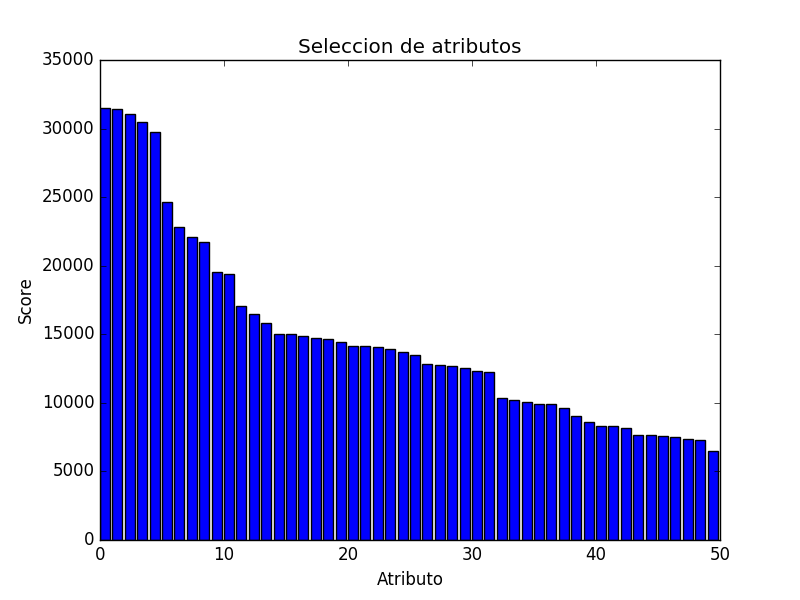
\includegraphics[height=8cm, width=10cm]{Seleccion_atributos.png}
\end{center}